%%%%% $Id: informe.tex $ %%%%%
\documentclass[10pt,a4paper]{article}
\usepackage[utf8]{inputenc}
\usepackage{amsmath}
\usepackage{amsfonts}
\usepackage{amssymb}
\usepackage{caratula}
\usepackage{listings}
\usepackage[pdftex,bookmarks=true,bookmarksnumbered=true,linkbordercolor={0 0 1},colorlinks=true,urlcolor=rltblue,linkcolor=rltred,citecolor=rltgreen,filecolor=blue]{hyperref}
\usepackage[pdftex]{graphicx, pdflscape}
\usepackage{color}
\usepackage{qtree}
\usepackage{multirow}


\lstset{
  basicstyle=\itshape,
  xleftmargin=3em,
  literate={->}{$\rightarrow$}{2}
           {λ}{$\lambda$}{1}
}

\begin{document}
\newpage

\materia{Teor\'ia de Lenguajes}
\submateria{Primer cuatrimestre 2013}
\titulo{TP Micro HTML Prettyprint}

\integrante{Ezequiel Gutesman}{715/02}{egutesman@gmail.com}
\integrante{Mauricio Alfonso}{65/09}{mauricioalfonso88@gmail.com}
\integrante{Victor Hugo Montero}{707/98}{vico.walker@gmail.com}

\maketitle
\newpage
\tableofcontents
\section{Primera Parte}
\subsection{Introducci\'on}


\paragraph{} Cuando comenzamos a pensar en cómo encarar el problema del desarrollo de la gramática, pensamos que podríamos tratar cada caracter (letra, número, espacio, etc.) como un símbolo terminal diferente, pero terminaríamos con una cantidad inmanejable de símbolos no terminales y producciones, es decir con una gramática enorme. Por esa razón definimos una serie de Token Léxicos que al pasárselos a un analizador léxico transforman el texto de entrada de una serie de caracteres en una serie de tokens.

\paragraph{} Definimos los tokens usando expresiones regulares. Primero definimos un token por cada tag de HTLM y por último un token para todo el texto que sobre. El analizador léxico tokeniza el archivo buscando los tokens en orden, de manera que todo el texto que halla entre dos tags queda tokenizado como \verb|texto|.

\paragraph{} El caso de la sección \verb|script| de HTML nos presentó un problema: entre los tags \verb|<script>| y \verb|</script>| puede haber cualquier combinación de caracteres excepto el tag de cierre de script. Esto quiere decir que podría haber incluso otros tags HTML dentro de un script, que deberían ser ignorados y que podrían no formar HTML válido. Pensamos en un principio en tokenizar el texto interior de los scripts con el analizador léxico como \verb|texto_sin_script| para tomar todo el texto que no tenga el tag \verb|</script>| como un token. Sin embargo no es posible tokenizar el texto de esta manera, ya que no tiene sentido poner el token \verb|texto_sin_script| antes ni después de los tags de HTML. 
Esto se debe a que si el analizador léxico busca primero el token \verb|texto_sin_script| y luego los tags, el primer token estaría ``absorviendo'' todos los tags excepto \verb|</script>| como parte de un script, incluso cuando no forman parte de un script; entonces no tokenizaría nunca los tags HTML. Si en cambio tokenizáramos primero los tags HTML y después \verb|texto_sin_script|, los tags del interior de los scripts serían reconocidos y el tag \verb|texto_sin_script| no cumpliría su función. Por esta razón decidimos tokenizar únicamente \verb|texto| para todo el texto que sobre luego de haber reconocido los tags HTML, y reconocer los tags que pueda haber en el script desde la gramática y no desde el analizador léxico.

\paragraph{} Además de tokenizar, el analizador léxico también se encarga de eliminar los comentarios y los espacios en blanco consecutivos, ya que estos podrían estar en cualquier parte del archivo recibido y debemos ignorarlos por completo.

\paragraph{} En la gramática definimos un símbolo no terminal $S$ para todo el documento.

\paragraph{} El símbolo no terminal $H$ contiene el interior del HTML, que a su vez puede tener un $HEAD$ y un $BODY$.

\paragraph{} Los símbolos $HEAD$ y $BODY$ representan las secciones head y body de HTML respectivamente, y los símbolos $HE$ y $B$ representan el interior de dichas secciones.

\paragraph{} Con el símbolo $SCS$ definimos una serie de cero o más scripts, que identificamos con el símbolo $SC$. 

\paragraph{} El símbolo $TSC$ representa el texto del interior de un script. Este es el símbolo con más producciones, ya que puede tener en su interior cualquier tag excepto \verb|</script>| y además estos pueden ir de cualquier manera, sin formar HTML válido.

\paragraph{} El interior de la sección body lo definimos recursivamente con el símbolo $B$, entendiendo que entre cada par de tags de apertura y cierre del mismo tipo puede haber más texto HTML válido.

\paragraph{} Decidimos que sólo puede haber un elemento \verb|<TITLE>...</TITLE>| dentro del head.

\subsection{Tokens L\'exicos}

\paragraph{} Los tokens l\'exicos est\'an descritos por expresiones regulares. La siguiente tabla describe para cada token su expresi\'on rgular correspondiente.


\begin{center}
    
\begin{tabular}{|l|l|}
\hline
\emph{Token L\'exico} & \emph{Expresi\'on Regular}\\
\hline \hline
\verb|<HTML>| & \texttt{<html>} \\
\verb|</HTML>| & \texttt{</html>}\\
\verb|<HEAD>| & \texttt{<head>}\\
\verb|</HEAD>| & \texttt{</head>}\\
\verb|<BODY>| & \texttt{<body>}\\
\verb|</BODY>| & \texttt{</body>}\\
\verb|<TITLE>| & \texttt{<title>}\\
\verb|</TITLE>| & \texttt{</title>}\\
\verb|<SCRIPT>| & \texttt{<script>}\\
\verb|</SCRIPT>| & \texttt{</script>}\\
\verb|<DIV>| & \texttt{<div>}\\
\verb|</DIV>| & \texttt{</div>}\\
\verb|<P>| & \texttt{<p>}\\
\verb|</P>| & \texttt{</p>}\\
\verb|<BR>| & \texttt{<br>}\\
\verb|texto| & \texttt{.*}\\
\hline
\end{tabular}

\end{center}
\paragraph{} Antes de tokenizar, el analizador l\'exico elimina espacios consecutivos y comentarios.
Los comentarios cumplen con la expresi\'on regular \verb|<!--.*-->|

\subsubsection{Correcciones Para la implementaci\'on}
Si bien la primer versi\'on de los tokens no ten\'ia ninguna corrección por parte del grupo docente, cambiamos la forma de tokenizar el token \verb|texto| dadas las posibilidades que nos brindaba ANTLR\footnote{www.antlr.org}. La nueva versi\'on del token qued\'o expresada como:

\verb|texto| & \texttt{[$\sim$<]*}\\
Queriendo representar cualquier caracter menos el s\'imbolo $<$


\subsection{Gram\'atica}
\label{sec:gramatica}
\paragraph{} La siguiente gram\'atica define el MicroHTML:

\[
    G = <N, \Sigma, P, S>
\]

Donde:
\begin{gather*}
    N = \{S, H, HEAD, BODY, HE, SCS, SC, TSC, B\}\\
    \Sigma = \{texto, <HTML>, </HTML>, <HEAD>, </HEAD>, \\
               <TITLE>, </TITLE>, <SCRIPT>, </SCRIPT>, \\
               <BODY>, </BODY>, <H1>, </H1>, <DIV>, </DIV>,\\
               <P>, </P>, <BR>\}\\
    S = S
\end{gather*}

\paragraph{} Que de acuerdo a la clasificaci\'on de Chomsky es una gram\'atica \emph{tipo 0}, o \emph{sin restricciones}. Las producciones ($P$) se detallan en la siguiente subsecci\'on.

\subsection{Producciones - $P$}
\begin{lstlisting}
S       -> <HTML> H </HTML>
 
H       -> HEAD BODY | HEAD | BODY | λ   

HEAD    -> <HEAD> HE </HEAD>

BODY    -> <BODY> B </BODY>

HE      -> SCS <TITLE> texto </TITLE> SCS 

SCS     -> SC SCS | λ

SC      -> <SCRIPT> TSC </SCRIPT>

TSC ->  <HTML> TSC | </HTML> TSC | 
        <HEAD> TSC | </HEAD> TSC |
        <BODY> TSC | </BODY> TSC |
        <TITLE> TSC | </TITLE> TSC |
        <DIV> TSC | </DIV> TSC |
        <H1> TSC | </H1> TSC |
        <P> TSC | </P> TSC |
        <SCRIPT> TSC | <BR> TSC | texto TSC | λ

B   ->  texto B |
        <DIV> B </DIV> B |
        <H1> B </H1> B |
        <P> B </P> B |
        <BR> B |
        λ

\end{lstlisting}


\subsubsection{Correcciones Para la implementaci\'on}

Debido a que ANTLR es un generador de parsers tipo LL(K) extendido, las producciones del símbolo no terminal H debieron ser cambiadas. En la gramática original dos de las producciones de H tienen el terminal \texttt{<HEAD>} como símbolo directriz, lo cual no está permitido en parsers LL. Las producciones de H fueron reemplazadas por una sola usando expresiones regulares de la siguiente manera:

\begin{lstlisting}
H       -> HEAD ? BODY ?
\end{lstlisting}

Por otra parte, para evitar que ANTLR reconozca cadenas inválidas formadas por HTML válido seguido de otros caracteres (por ejemplo \\ \texttt{<html></html>aaa}), fue necesario agregar el símbolo de fin de archivo (EOF en ANTLR) a la producción del símbolo distinguido S, quedando de la siguiente manera:

\begin{lstlisting}
S       -> <HTML> H </HTML> $
\end{lstlisting}

\subsection{Arbol de derivaci\'on}

\paragraph{} A continuaci\'on presentamos el \'arbol de derivaci\'on para el siguiente ejemplo:

\begin{verbatim}
<HTML>
    <HEAD>
        <TITLE>Una pagina de ejemplo</TITLE>
        <SCRIPT>
        function unaFunc(){
            alert("esta funcion imprime un tag roto <TITLE>");
        }
        </SCRIPT>
        <SCRIPT></SCRIPT>
        <SCRIPT>alert("aca no aparece el cierre de SCRIPT")</SCRIPT>
    </HEAD>
    <BODY>
        <H1>Un heading</H1>
        <DIV>
            <P>Este texto es de prueba</P>
        </DIV>
        <BR>
        <P>Mas prueba</P>
    </BODY>
</HTML>
\end{verbatim}

\paragraph{} Debido al tamaño del ejemplo, el árbol de derivación tuvo que ser partido en dos partes. Nótese que del (único) nodo con el no terminal $H$ cuelgan 2 hijos con el no-terminal $HEAD$, y el no terminal $BODY$. El primer subárbol muestra los descendientes de $HEAD$ y el segundo los de $BODY$. En cada árbol, el no terminal cuyo subárbol está suprimido se encuentra marcado en rojo, y con un subárbol genérico (triangulo) simbolizando que en realidad continúa. Por ejemplo:

\begin{enumerate}
\qtreecenterfalse
\item[] a.
 \Tree  [.\textbf{H} 
            [\qroof{desarrollado}.{\textbf{$HEAD$}} ]
            [\qroof{\color{red}suprimido}.{\textbf{\color{red}$BODY$}} ] 
        ] 
        \hskip 0.3in
 b.
 \Tree  [.\textbf{H} 
            [\qroof{\color{red}suprimido}.{\textbf{\color{red}$HEAD$}} ]
            [\qroof{desarrollado}.{\textbf{$BODY$}} ] 
        ]
 \end{enumerate}

En la figura \emph{a.} se suprime el subárbol corrspondiente al no terminal $BODY$ y en el \emph{b.} el correspondiente al no terminal $HEAD$. 


\begin{landscape}

\hspace*{-0.1\linewidth}\resizebox{1.1\linewidth}{!}{%
\Tree [.S 
        [.$<HTML>$ ] 
        [.\textbf{H} 
            [.HEAD 
                [$<HEAD>$ ] 
                [.HE 
                     [.SCS 
                         [.$\lambda$ ]                          
                     ] 
                     [.$<TITLE>$ ] 
                     [.texto ] 
                     [.$</TITLE>$ ] 
                     [.SCS 
                         [.SC
                              [.$<SCRIPT>$ ]  
                              [.TSC 
                                  [.texto ] 
                                  [.TSC 
                                      [.$<TITLE>$ ] 
                                      [.TSC 
                                          [.texto ] 
                                          [.TSC 
                                              [.$\lambda$ ] 
                                          ]                                          
                                      ]   
                                  ] 
                              ] 
                              [.</SCRIPT> ] 
                         ] 
                         [.SCS 
                             [.SC 
                                 [.$<SCRIPT>$ ] 
                                 [.texto ] 
                                 [.$</SCRIPT>$ ]
                             ] 
                             [.SCS 
                                 [.SC 
                                     [.$<SCRIPT>$ ] 
                                     [.texto ]
                                     [.$</SCRIPT>$ ] 
                                 ] 
                                 [.SCS 
                                     [.$\lambda$ ] 
                                 ]                                 
                             ]
                         ]
                     ] 
                ] 
                [.$</HEAD>$ ]
            ]
            [\qroof{\color{red}suprimido}.{\textbf{\color{red}$BODY$}} ]
        ]
        [.$</HTML>$ ] 
    ].S
}


\hspace*{-0.1\linewidth}\resizebox{1.1\linewidth}{!}{%
\Tree [.S 
        [.$<HTML>$ ] 
        [.\textbf{H} 
            [\qroof{\color{red}suprimido}.{\textbf{\color{red}$HEAD$}}  ]
            [.BODY 
                [.$<BODY>$ ] 
                [.B 
                    [.$<H1>$ ]
                    [.B 
                        [.texto ] 
                        [.B 
                            [.$\lambda$ ]
                        ] 
                    ]
                    [.$</H1>$ ]
                    [.B 
                        [.$<DIV>$ ]
                        [.B 
                            [.$<P>$ ]
                            [.B 
                                [.texto ]
                                [.B 
                                    [.$\lambda$ ]
                                ]
                            ]
                            [.$</P>$ ]
                        ]
                        [.$</DIV>$ ]
                        [.B
                            [.$<BR>$ ]
                            [.B
                                [.$<P>$ ]
                                [.B 
                                    [.texto ]
                                    [.B 
                                        [.$\lambda$ ]
                                    ]
                                ]
                                [.$</P>$ ]
                            ]
                        ]
                    ] 
                ] 
                [.$</BODY>$ ] 
            ]
        ]
        [.$</HTML>$ ]
    ].S
}
\end{landscape}
\section{Segunda Parte}
\subsection{Implementaci\'on}
\subsubsection{Descripci\'on del problema}
Se pidió en esta segunda parte implementar un parser que parsee texto según la gramática especificada en la sección \ref{sec:gramatica}. Esta implementación debería tomar como entrada una cadena de texto y en caso de poder parsearla, producir como salida un archivo en formato HTML que se pueda abrir desde un browser y que dentro de él, se encuentre el texto procesado de la entrada pero correctamente indentado y coloreado.

Por ejemplo, para la siguiente entrada:

      \begin{verbatim}
<html><head><title>Título</title><script>print("hello")</script>
</head><body>texto<p>párrafo<h1><!--comentario--><p> más texto
</p></h1></p> <div>texto texto texto <br> mas texto texto texto
</div> </body> </html>\end{verbatim}

Se producirá la siguiente salida en un archivo HTML:

\begin{figure}[h!]
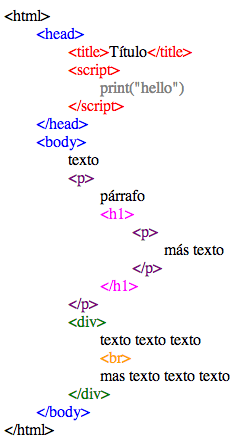
\includegraphics[width=5cm]{img/ejemplo1.png}
      \caption{Salida para un ejemplo válido.}
      \label{tbl:ejemplo}
\end{figure}

\newpage
\subsubsection{Detalles de implementación y limitaciones}
La solución fue desarrollada con ANTLR\footnote{www.antlr.org} y tanto el lexer como el parser fueron generados en Java.

El parser no acepta el símbolo \verb|<| dentro de un tag script. Esto podría tokenizarse mejor ya que una comparación dentro del script haría que falle el parsing.

En cuanto a la salida del parsing, esta es calculada en un atributo \textbf{sintetizado} llamado \texttt{texto}. Para manejar la indentación, utilizamos un único tag \verb|<div class="bloque">| cuyo único estilo tiene un margen a izquierda, fijo. El efecto de ir generando estos divs a medida que se necesita generar un tag produce la indentación deseada, contemplando el nivel de encadenamiento de tags producto de ir procesando un tag dentro de otro.

En cuanto al coloreo de los tags, cada tag reconocido tiene su correspondiente código HTML con un estilo (CSS) que le otorga el color.

\subsubsection{Entradas de prueba válidas}

\underline{Entrada 1:}
\begin{verbatim}
<html><head><title>Título</title><script>print("hello")</script>
</head><body>texto<p>párrafo<h1><!--comentario--><p> más texto
</p></h1></p> <div>texto texto texto <br> mas texto texto texto
</div> </body> </html>\end{verbatim}

\underline{Salida 1:}

\begin{figure}[h!]
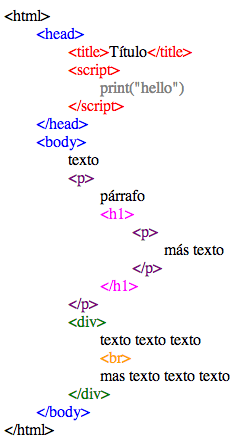
\includegraphics[width=4.7cm]{img/ejemplo1.png}
      \caption{Salida para un ejemplo válido.}
      \label{salida1}
\end{figure}

\newpage

\underline{Entrada 2:}

\begin{verbatim}
<html>  <head> <script>print("a script")</script><title>Título</title>
 <script>print("hello")</script><script>print("world")</script>
</head><body>texto suelto<p>párrafo <h1><!-- comentario--><p> más texto</p></h1>
</p><div>texto texto texto <br> mas texto textotexto</div><div>
Un Div que adentro tiene otro<div>Dentro <div><p>de otro</p> con mas texto
</div></div></div>  </body>  </html>
\end{verbatim}

\underline{Salida 2:}

\begin{figure}[h!]
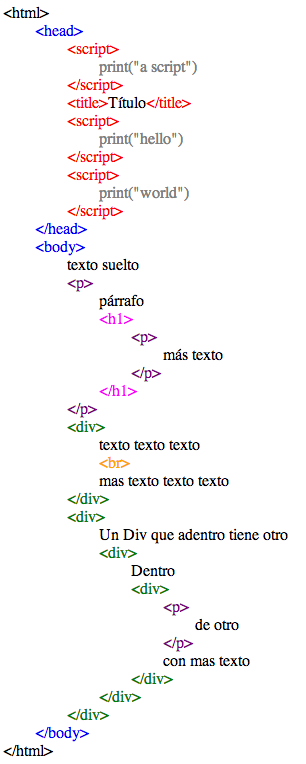
\includegraphics[width=6.2cm]{img/ejemplo2.png}
      \caption{Salida para un ejemplo válido.}
      \label{salida2}
\end{figure}

\newpage 

\subsubsection{Entradas de prueba inválidas}

\underline{Entrada 3 (\texttt{<title>} sin abrir):}
\begin{verbatim}
<html>  Título</title> <script>print("hello")</script><script>print("world")
</script></head><body>texto suelto<p>párrafo <h1><!-- comentario--><p> 
más texto</p></h1></p><div>texto texto texto <br> mas texto texto texto
</div><div>Un Div que adentro tiene otro<div>Dentro <div><p>de otro
</p> con mas texto</div></div></div></body></html>
	\end{verbatim}
    
\underline{Salida 3:}
\\\\
\verb|line 1:6 missing TK_C_HTML at ' Título' <html>|\\\\
\underline{Entrada 4 (\texttt{<div>} sin cerrar):}
\\\\
\begin{verbatim}
<html>  <head> <script>print("a script")</script><title>Título</title>
<script>print("hello")</script><script>print("world")</script>
</head><body>texto suelto<p>párrafo <h1><!-- comentario--><p> 
más texto</p></h1></p><div>texto texto texto <br> mas texto texto 
texto<div>Un Div que adentro tiene otro<div>Dentro <div><p>de otro</p> 
con mas texto</div></div></div></body></html>
\end{verbatim}

\underline{Salida 4:}\\\\
{\footnotesize
\verb|line 6:0 mismatched input '<span class="body">&lt;/body&gt;</span>' expecting TK_C_DIV|
}

\subsection{Conclusiones}
\paragraph{}El problema que el presente trabajo resuelve sirvi\'o como caso de estudio para el desarrollo, en la primera etapa, de una gram\'atica \emph{sin restricciones} (seg\'un la clasificaci\'on de Chomsky). En esa primera etapa tuvimos que tomar decisiones sobre c\'omo tokenizar la versi\'on reducida del lenguaje HTML para poder generar, dada una cadena de texto, la versi\'on correctamente coloreada e indentada, siempre y cuando esta formaba una entrada HTML v\'alida.

\paragraph{}La primer parte del trabajo no present\'o mayores dificultades mas all\'a de la toma de decisiones referentes a qu\'e parte del parsing ser\'ia manejado con producciones en la gram\'atica y cuales con la tokenizaci\'on. 

\paragraph{}En una segunda parte desarrollamos una implementaci\'on en el lenguaje Java, utilizando el generador de parsers \emph{ANTLR}. La gram\'atica desarrollada no ten\'ia mayores problemas estructurales, por lo tanto procedimos a la sintetizaci\'on de atributos dentro de \emph{ANTRL}. Luego de una primera entrega, se reportaron errores atribu\'idos principalmente a dos problemas dentro de la implementaci\'on:

\begin{enumerate}
    \item La salida del parsing era emitida como salida a medida que se sintetizaban los atributos y se parseaba la entrada, esto produjo que para entradas inv\'alidas haya una salida parcial, interrumpida en el momento de emitir un error. 
    \item Permitir saltos de l\'inea dentro de los tags HTML procesaba como v\'alidos aquellas cadenas de texto donde los tags estaban separados entre 2 o m\'as lineas. 
\end{enumerate}

\paragraph{}Ambos errores fueron corregidos y la implementaci\'on entregada no posee estos problemas.

\paragraph{}En cuanto a \emph{ANTLR} result\'o ser basntante intuitiva la manera en la que se sintetizan atributos a medida que se realiza el parsing de la entrada. El uso del lenguaje Java dentro de los bloques de c\'odigo donde se realiza la sintetizaci\'on otorgan una felixibilidad notable que imaginamos facilita el desarrollo de parsers de mayor complejidad.

\paragraph{}Hubiera sido interesante comparar una implementaci\'on del mismo parser en tecnolog\'ias como \emph{Bison}\footnote{http://www.gnu.org/software/bison/} o \emph{Lex, YACC}\footnote{http://dinosaur.compilertools.net/}. Principalmente porque estos generan parsers LALR a diferencia de \emph{ANTLR} que genera parsers LL(*). Podríamos haber tomado otras decisiones en la gram\'atica y analizar su impacto en la performance de los parsers. Por ejemplo, una gram\'atica recursiva a izquierda no habr\'ia sido soportada por \emph{ANTLR} pero s\'i por \emph{YACC} y \emph{Bison}. Este tipo de comparaci\'on comprende un trabajo mayor tanto en la escritura de las gram\'aticas como en las implementaciones.
\subsection{Apendice - Código}
\texttt{prettyprint.g}
{\tiny
\begin{verbatim}
grammar prettyprinter;

options {
    language = Java;
    output = AST;
}


/* *********** PRODUCCIONES *********** */

s returns [String texto]
  : t1=TK_HTML h1=h t2=TK_C_HTML EOF {
      $texto = 
          "<html><head>" + 
          "<style type=\"text/css\">" + 
          "div.bloque {margin-left: 2em;}" + 
          "span.html {color:black;}" +
          "span.p {color:purple;}" +
          "span.head {color:blue;}" +
          "span.body {color:blue;}" +
          "span.title {color:red;}" +
          "span.script_tag {color:red;}" +
          "span.script {color:grey;}" +
          "span.h1 {color:fuchsia;}" +
          "span.div {color:green;}" +
          "span.br {color:orange;}" +
          "</style>" +
          "</head><body>" +
          $t1.getText() + $h1.texto + $t2.getText() + 
          "</body></html>"
      ;
  };
  
h returns [String texto]
  : {$texto = "";} 
    (h1=head {$texto += $h1.texto;})? 
    (b1=body {$texto += $b1.texto;})?
  ;

head returns [String texto]
  : t1=TK_HEAD h1=he t2=TK_C_HEAD {
      $texto = "<div class=\"bloque\">" + $t1.getText() + $h1.texto 
      + $t2.getText() + "</div>";
  };

body returns [String texto]
  : t1=TK_BODY b1=b t2=TK_C_BODY {
      $texto = "<div class=\"bloque\">" + $t1.getText() + $b1.texto 
      + $t2.getText() + "</div>";
  };
  
he returns [String texto]
  : sc1=scs t1=TK_TITLE t2=TK_TEXTO t3=TK_C_TITLE scs2=scs {
      $texto = $sc1.texto + "<div class=\"bloque\">" + $t1.getText() 
      + $t2.getText() + $t3.getText() + "</div>" + $scs2.texto;
  };

scs returns [String texto]
  : sc1=sc scs1=scs {$texto = $sc.texto + $scs1.texto;}
  | {$texto = "";}  //lambda
  ; 

sc returns [String texto]
  : t1=TK_SCRIPT ts=tsc t2=TK_C_SCRIPT {
      $texto = "<div class=\"bloque\">" + $t1.getText() + "<div class=\"bloque\">"
      + "<span class=\"script\">" + $ts.texto + "</span>" + "</div>" + $t2.getText() + "</div>";
  };  

tsc returns [String texto]
  : (
      tk=TK_HTML ts=tsc | tk=TK_C_HTML ts=tsc
    | tk=TK_HEAD ts=tsc | tk=TK_C_HEAD ts=tsc
    | tk=TK_BODY ts=tsc | tk=TK_C_BODY ts=tsc
    | tk=TK_TITLE ts=tsc | tk=TK_C_TITLE ts=tsc
    | tk=TK_DIV ts=tsc | tk=TK_C_DIV ts=tsc   
    | tk=TK_H1 ts=tsc | tk=TK_C_H1 ts=tsc    
    | tk=TK_P ts=tsc | tk=TK_C_P ts=tsc
    | tk=TK_SCRIPT ts=tsc
    | tk=TK_BR ts=tsc
    | tk=TK_TEXTO ts=tsc
   ) {$texto = $tk.getText() + $ts.texto;}
  | {$texto = "";} //lambda
  ;
  
b returns [String texto]
  : t1=TK_TEXTO b1=b {
        $texto = "<div class=\"bloque\">" + $t1.getText()  + "</div>" + $b1.texto;
    }
  | t1=TK_DIV b1=b t2=TK_C_DIV b2=b {
        $texto = "<div class=\"bloque\">" + $t1.getText() + $b1.texto 
        + $t2.getText() + "</div>" + $b2.texto;
    }
  | t1=TK_H1 b1=b t2=TK_C_H1 b2=b {
        $texto = "<div class=\"bloque\">" + $t1.getText() + $b1.texto 
        + $t2.getText() + "</div>" + $b2.texto;
    }
  | t1=TK_P b1=b t2=TK_C_P b2=b {
        $texto = "<div class=\"bloque\">" + $t1.getText() + $b1.texto 
        + $t2.getText() + "</div>" + $b2.texto;
    }
  | t1=TK_BR b1=b {
        $texto = "<div class=\"bloque\">" + $t1.getText()  + "</div>" + $b1.texto;
    } 
  | {
        $texto = "";  //lambda
  }; 
  

/* *********** TOKENS *********** */

WS : (' ' | '\t' | '\r' | '\n')+ {
    $channel = HIDDEN;  //para ignorar los blancos
}; 
      
COMM : '<!' .* '>' {
    $channel = HIDDEN;  //para ignorar comentarios
};               

TK_HTML returns [String texto]: '<html>' {
    setText("<span class=\"html\">&lt;html&gt;</span>");
};

TK_C_HTML returns [String texto]: '</html>' {
    setText("<span class=\"html\">&lt;/html&gt;</span>");
};

TK_HEAD : '<head>' {
    setText("<span class=\"head\">&lt;head&gt;</span>");
};

TK_C_HEAD : '</head>' {
    setText("<span class=\"head\">&lt;/head&gt;</span>");
};

TK_TITLE : '<title>' {
    setText("<span class=\"title\">&lt;title&gt;</span>");
};

TK_C_TITLE : '</title>' {
    setText("<span class=\"title\">&lt;/title&gt;</span>");
};

TK_SCRIPT : '<script>' {
    setText("<span class=\"script_tag\">&lt;script&gt;</span>");
};

TK_C_SCRIPT : '</script>' {
    setText("<span class=\"script_tag\">&lt;/script&gt;</span>");
};

TK_BODY : '<body>' {
    setText("<span class=\"body\">&lt;body&gt;</span>");
};

TK_C_BODY : '</body>' {
    setText("<span class=\"body\">&lt;/body&gt;</span>");
};

TK_H1 : '<h1>' {
    setText("<span class=\"h1\">&lt;h1&gt;</span>");
};

TK_C_H1 : '</h1>' {
    setText("<span class=\"h1\">&lt;/h1&gt;</span>");
};

TK_DIV : '<div>' {
    setText("<span class=\"div\">&lt;div&gt;</span>");
};

TK_C_DIV : '</div>' {
    setText("<span class=\"div\">&lt;/div&gt;</span>");
};

TK_P : '<p>' {
    setText("<span class=\"p\">&lt;p&gt;</span>");
};

TK_C_P : '</p>' {
    setText("<span class=\"p\">&lt;/p&gt;</span>");
};

TK_BR : '<br>' {
    setText("<span class=\"br\">&lt;br&gt;</span>");
};

TK_TEXTO : (~('<'))+;  //todo menos <

\end{verbatim}
}




\end{document}

